\documentclass[11pt,a4paper]{article}
\usepackage{cite}
\usepackage{color}
\usepackage{graphicx}
\usepackage{amsmath}
\usepackage[margin=1in]{geometry}
\usepackage{listings}
\usepackage{hyperref}

\title{The DJH INS ROS Package Documentation}
\author{David Hanley, Alex Faustino, David Degenhardt, Tim Bretl}

\begin{document}
\maketitle

\begin{abstract}
	The purpose of this article is to document the approach to the DJH inertial navigation system (INS) ROS package. This package, we anticipate, will be used in a variety of other navigation systems. For example, we design this so that it can be easily used in a visual-inertial odometry system or a magnetic positioning system.
\end{abstract}

\section{Introduction}

The DJH INS ROS package is designed to provide several potentially useful computations to a user as IMU data is received. These include:
\begin{itemize}
	\item IMU data aggregated into sets of Eigen matrices
	\item blah blah blah
\end{itemize}

\section{The IMU Aggregator}

One of the functions of the DJH INS is that an INS solution is only computed when requested by the $\texttt{comp\_sol}$ topic. This topic is a message created for this package that includes:
\begin{itemize}
	\item $\texttt{Header	header}$
	\item $\texttt{float64	time\_desired}$
	\item $\texttt{bool		stop\_agg}$
\end{itemize}
The $\texttt{time\_desired}$ variable is the time for which an INS solution is desired. The $\texttt{stop\_agg}$ variable is switched to $\texttt{true}$ when it is desired to stop aggregating the data (presumably to then compute an INS solution at $\texttt{time\_desired}$). As the system is running if IMU data is collected with a timestamp at or after $\texttt{time\_desired}$, then that data is saved for use in a matrix with a later $\texttt{time\_desired}$. The aggregated matrix is published on a topic called $\texttt{aggregate\_imu}$. This aggregated IMU data is published as Float64 vector standard message in ROS. The following C++ code shows how to convert that message into a regular $n$-by-7 Eigen matrix.
\begin{lstlisting}[frame=single,breaklines] [language=c++]
    /*------- Receive and reform aggregated IMU Matrix -------*/
    // Define a temporary std vector for the aggregated IMU 
    // message data
    vector<double> vec = msg->data;
    // Compute the number of rows in the aggregated matrix
    int sz = vec.size()/7;
    // Create pointer and store memory address of first vector element
    double* ptr = &vec[0];
    // Note: MatrixX7d is defined in aggregator.h
    Map<MatrixX7d>agg_mat(ptr,sz,7);
    /*----- End receive and reform aggregated IMU Matrix -----*/

    // Print Results
    cout << "-----------------------------------------------\n";
    cout << agg_mat << endl;
    cout << "-----------------------------------------------\n";
\end{lstlisting}
The structure of the resulting aggregated matrix is as follows:
\begin{equation}
	\left[\begin{array}{ccccccc}
		timestamp_1 & accel_{x1} & accel_{y1} & accel_{z1} & gyro_{x1} &  gyro_{y1} & gyro_{z1} \\
		timestamp_2 & accel_{x2} & accel_{y2} & accel_{z2} & gyro_{x2} &  gyro_{y2} & gyro_{z2} \\
		... & ... & ... & ... & ... & ... & ...
	\end{array}\right]
\end{equation}
Since the DJH INS package is a ROS node, it can interface with some navigation algorithm through ROS topics. Using $\texttt{bare\_bones\_node}$ as an example navigation node (such as a visual-inertial odometry code), the aggregated IMU data can interface with it as shown in Figure \ref{fig:djhinsagg}.


\begin{figure}
	\centering
	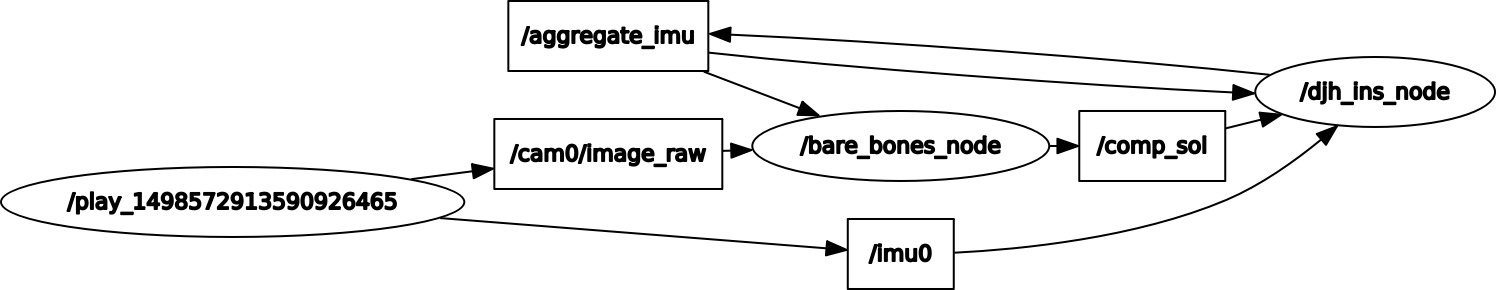
\includegraphics[scale=0.425]{djhinsagg}
	\caption{The DJH INS package receives IMU data and a flag to stop aggregating that IMU data in a matrix. That aggregated data is then published and can be used by both the $\texttt{djh\_ins\_node}$ for computing an INS solution or by some other node (in this case $\texttt{bare\_bones\_node}$) for some other reason.}
	\label{fig:djhinsagg}
\end{figure}

\section{The IMU Model and Corrector}

The elements of the aggregated matrix are corrected for fixed scale factors ($S_g$ and $S_a$), cross-coupling effects ($M_g$ and $M_a$), and biases ($B_{fg}$ and $B_{fa}$). These parameters (since they are fixed) are set in a parameter file called $\texttt{IMUmodel.yaml}$. We also assume that the navigation algorithm can potentially estimate some bias online ($B_g$ for the gyroscopes and $B_a$ for the accelerometers). Therefore, we have set up a subscriber to a ROS topic called $\texttt{bias\_est}$ which contains a $\texttt{std\_msgs::Float64MultiArray}$ message. The first three elements of the message are assumed to correspond to the x, y, and z-axis accelerometer biases respectively. The second three elements of the message are assumed to correspond to the x, y, and z-axis gyroscope biases respectively. Equations \ref{fig:gyrocorrect} and \ref{fig:accelcorrect} show how we use measurements from the gyroscopes, $\omega$, and accelerometers, $a_{sf}$, to compute corrected gyroscope, $\tilde{\omega}$, and accelerometer, $\tilde{a}_{sf}$, data. Figure \ref{fig:withonlinebias} shows the same information as Figure \ref{fig:accelcorrect}. However, now ROS topics relevant for IMU error correction is also included.

\begin{equation}
	\tilde{\omega} = (1 + S_g)\omega + M_g \omega + B_{fg} + B_g
	\label{fig:gyrocorrect}
\end{equation}

\begin{equation}
	\tilde{a}_{sf} = (1 + S_a)a_{sf} + M_a a_{sf} + B_{fa} + B_a
	\label{fig:accelcorrect}
\end{equation}

\begin{figure}
	\centering
	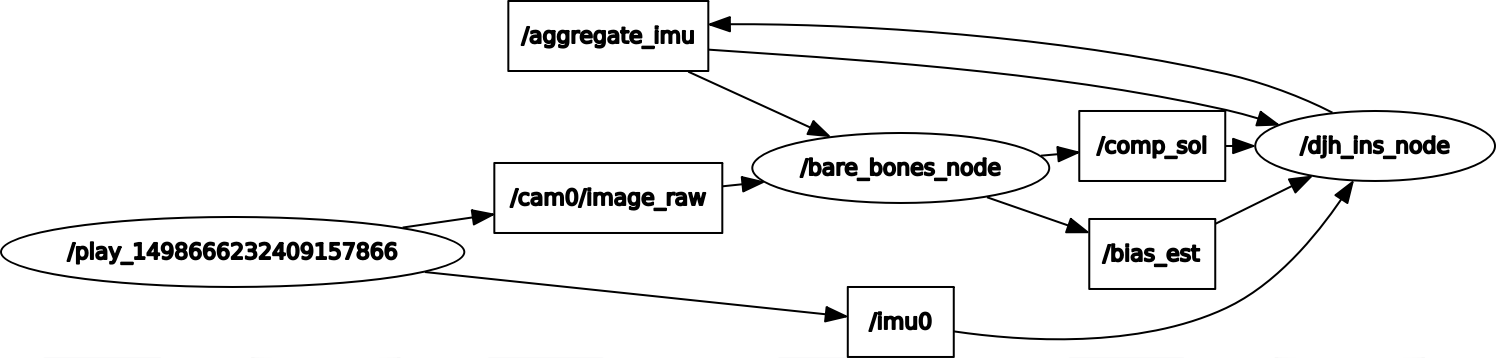
\includegraphics[scale=0.42]{withonlinebias}
	\caption{This ROS graph shows all the ROS topics associated with aggregating IMU data and with correcting IMU measurements.}
	\label{fig:withonlinebias}
\end{figure}

\section{Quaternion Math Library}

Our INS code makes significant use of the C++ library Eigen (\url{http://eigen.tuxfamily.org}). However, we do not make use of Eigen's quaternion functionalities. This is because we use a JPL convention for quaternions. More information on the JPL convention can be found at \cite{Trawny:2005,Barfoot:2011,Wie:2008}. There we create our own quaternion math class call $\texttt{QuatMath}$ which performs the following functions on JPL-style quaterions:
\begin{itemize}
	\item[1] Normalize the Quaternion
	\item[2] Compute the Angle of Rotation
	\item[3] Perform Quaternion Multiplication
	\item[4] Compute the Quaternion Inverse
	\item[5] Create a Rotation Matrix from a Quaternion
	\item[6] Convert Rotation Matrix to a Quaterion.
\end{itemize}

\section{Integration Algorithms and Implementation}

\section{Conclusion}

blah blah blah \cite{Forster:2017,Forster:2015,Eckenhoff:2016}

\bibliographystyle{IEEEtran}
\bibliography{IEEEabrv,references}

\end{document}